\chapter{Greedy structure: true for \texorpdfstring{$k=3$}{k=3}, false for \texorpdfstring{$k\ge4$}{k>=4}}\label{sec:greedy}

For $k=3$ the decision problem can be solved in near-linear
time~\citep{tw25}, and $O(n^2)$ time suffices for the optimisation
problem~\citep{kobayashi}. These algorithms exploit that an $r$-far triple, if
one exists, can be found next to the ``first far points'' of some point. It is
natural to ask how much of this structure survives for larger $k$, because any
property of this kind immediately yields a fast greedy or bounded-search
algorithm. This section gives a complete answer for the properties we are
aware of.

Fix $r>0$. For $q\in P$ let $a(q)$ be the first point after $q$ in ccw order
with $|q\,a(q)|\ge r$, and $b(q)$ the first such point in clockwise order;
both are undefined if no point is at distance at least $r$ from $q$. Note that
the distance from $q$ is in general not unimodal along the hull, so points
after $a(q)$ may again be close to $q$. Let $\Arc(q)$ be the set of points on
the ccw arc from $a(q)$ to $b(q)$ (which does not contain $q$). We call
$\{q,a(q)\}$ a \emph{tight pair}.

\begin{lemma}\label{lem:arcbasic}
Let $S$ be an $r$-far set with $|S|\ge2$, and let $s,s'$ be consecutive points
of $S$ in ccw order. Then $a(s)$ lies in $P(s,s')\cup\{s'\}$, and
$S\setminus\{s\}\subseteq\Arc(s)$.
\end{lemma}
\begin{proof}
All points of $S\setminus\{s\}$ are at distance at least $r$ from $s$; the first
of them in ccw order is $s'$ and the first in clockwise order is the
predecessor of $s$ in $S$.
\end{proof}

We consider the following properties of $(P,k,r)$.
\begin{description}[leftmargin=3.2em,labelwidth=2.6em,itemsep=2pt]
\item[$(\mathrm{G}_k)$] \emph{Arc characterisation:} $P$ has an $r$-far $k$-set
if and only if $\Arc(q)$ contains an $r$-far $(k-1)$-set for some $q\in P$.
\item[$(\mathrm{TT}_k)$] \emph{Tight triple:} if $P$ has an $r$-far $k$-set,
then it has one that contains $q$, $a(q)$ and $b(q)$ for some $q$.
\item[$(\mathrm{TP}_k)$] \emph{Tight pair:} if $P$ has an $r$-far $k$-set, then
it has one that contains a tight pair $\{q,a(q)\}$.
\item[$(\mathrm{ST}_k)$] \emph{Seeded search tree:} if $P$ has an $r$-far $k$-set, then
for some $q$ the following search reaches $k$ points: start with
$\{q,a(q)\}$, a ccw frontier at $a(q)$ and a clockwise frontier at $q$, and
repeatedly add, on a side of the search's choice, the first point beyond that
side's frontier (and before the other frontier) that is at distance at least
$r$ from all chosen points; the added point becomes the new frontier.
\item[$(\mathrm{AG}_k)$] \emph{Alternating greedy:} as $(\mathrm{ST}_k)$, but
the sides strictly alternate (either side may start).
\end{description}
Every set produced by a search of $(\mathrm{ST}_k)$ is $r$-far and contains
$\{q,a(q)\}$, so
$(\mathrm{AG}_k)\Rightarrow(\mathrm{ST}_k)\Rightarrow(\mathrm{TP}_k)$, and
trivially $(\mathrm{TT}_k)\Rightarrow(\mathrm{TP}_k)$. If $(\mathrm{ST}_k)$ held
for all point sets, the decision problem could be solved in $O(2^kn^2k)$ time
by exploring, for each of the $n$ seeds, a binary tree of depth $k-2$ whose
nodes cost $O(nk)$; $(\mathrm{AG}_k)$ would even give $O(n^2k)$. Property
$(\mathrm{TP}_k)$ is the weakest statement that ties a solution to the first
far points, and therefore the most robust candidate. The bounded search tree
of Singireddy, Basappa and Mitchell~\citep{sbm} is a two-sided variant of
$(\mathrm{ST}_k)$ that is seeded with a single point; we study it separately
in \cref{sec:sbm}.

\section{Triples}\label{sec:k3}

\begin{theorem}\label{thm:k3}
Let $\{x,y,z\}$ be an $r$-far triple of $P$, in ccw order.
\begin{enumerate}[label=(\roman*),itemsep=1pt,topsep=2pt]
\item At least one of $\{x,a(x),b(x)\}$, $\{y,a(y),b(y)\}$,
$\{z,a(z),b(z)\}$ is an $r$-far triple.
\item At least one of $\{x,a(x),z\}$, $\{y,a(y),x\}$, $\{z,a(z),y\}$ is an
$r$-far triple.
\end{enumerate}
In particular $(\mathrm{TT}_3)$, $(\mathrm{TP}_3)$, $(\mathrm{ST}_3)$ and
$(\mathrm{AG}_3)$ hold for every point set in convex position and every $r$.
\end{theorem}
\begin{proof}
(i) By \cref{lem:arcbasic}, the ccw order around the hull is
$x,a(x),y,z,b(x)$, where $a(x)=y$ and $b(x)=z$ are allowed, and
$a(x)\ne b(x)$. Suppose that $|a(x)b(x)|<r$. In the triangle $x\,a(x)\,b(x)$
the side $a(x)b(x)$ is then strictly shorter than the other two, so the
opposite angle is smaller than $\pi/3$, and by (A),
$\ang yxz\le\ang a(x)\,x\,b(x)<\pi/3$. If the triples of $y$ and $z$ also
failed to be $r$-far, the same argument would give $\ang zyx<\pi/3$ and
$\ang xzy<\pi/3$, and the angles of the triangle $xyz$ would sum to less than
$\pi$.

(ii) If $a(x)=y$ the first triple is $\{x,y,z\}$. Otherwise $a(x)\in P(x,y)$
and $|x\,a(x)|\ge r$, so the first triple is $r$-far unless $|a(x)z|<r$. In
that case $a(x)z$ is the strictly shortest side of the triangle $x\,a(x)\,z$,
hence $\ang a(x)\,x\,z<\pi/3$, and by (A) applied to $x,a(x),y,z$ we get
$\ang yxz<\pi/3$. Likewise, failure of the second triple gives
$\ang zyx<\pi/3$ and failure of the third gives $\ang xzy<\pi/3$. All three
cannot fail.

The tight triple of (i) contains the tight pair $\{q,a(q)\}$. For
$(\mathrm{ST}_3)$ and $(\mathrm{AG}_3)$, take the triple $\{q,a(q),z'\}$
provided by (ii): the search started from $\{q,a(q)\}$ needs a single step,
and its ccw step succeeds because the arc beyond $a(q)$ contains a point,
namely $z'$, at distance at least $r$ from both seeds.
\end{proof}

Part~(i) says that $P$ has an $r$-far triple if and only if
$|a(q)b(q)|\ge r$ for some $q$, a characterisation in the spirit of the
fast algorithms for $k=3$~\citep{kobayashi,tw25}; we include the proof
because it is short and because part~(ii) uses the same idea. The arc
characterisation holds for triples as well.

\begin{proposition}\label{prop:g3}
The implication ``$\Rightarrow$'' of $(\mathrm{G}_k)$ holds for every
$k\ge2$, and $(\mathrm{G}_3)$ holds.
\end{proposition}
\begin{proof}
If $S$ is an $r$-far $k$-set and $q\in S$, then $S\setminus\{q\}$ is an
$r$-far $(k-1)$-set contained in $\Arc(q)$ by \cref{lem:arcbasic}.

For $k=3$, let $x,y\in\Arc(q)$ with $|xy|\ge r$, write $a=a(q)$, $b=b(q)$,
and let the ccw order be $q,a,x,y,b$ with $a=x$ or $y=b$ allowed. Suppose that
$P$ has no $r$-far triple. Since $a\ne b$ and $|qa|,|qb|\ge r$, we have
$|ab|<r$. We distinguish cases according to the distances from $q$.
If $|qx|\ge r$ and $|qy|\ge r$, then $\{q,x,y\}$ is an $r$-far triple.
If $|qx|<r\le|qy|$, then $x\ne a$, and $|ay|<r$ because $\{q,a,y\}$ is not
$r$-far. In the convex quadrilateral $q,a,x,y$ the diagonals satisfy
$|qx|+|ay|<2r\le|qa|+|xy|$, contradicting~(Q). The case $|qy|<r\le|qx|$ is
symmetric: $y\neq b$, $|xb|<r$, and the quadrilateral $q,x,y,b$ has diagonals
$|qy|+|xb|<2r\le|xy|+|bq|$. Finally, if $|qx|<r$ and $|qy|<r$, then, as in the
proof of \cref{thm:k3}, $\ang xqy\le\ang aqb<\pi/3$, so $xy$ is not a longest
side of the triangle $qxy$ and $|xy|<\max\{|qx|,|qy|\}<r$, a contradiction.
\end{proof}

\section{Four or more points}\label{sec:k4}

\begin{proposition}\label{prop:gk}
$(\mathrm{G}_k)$ fails for every $k\ge4$: there is a set of $k$ points in
convex position and a radius $r$ such that no $r$-far $k$-set exists although
$\Arc(u)$ contains an $r$-far $(k-1)$-set for some point $u$.
\end{proposition}
\begin{proof}
Let $k\ge4$, choose $k-2$ distinct non-zero integers $j$ with $|j|\le k$, at
least one positive and one negative, and let $H=3(k+1)$. Let
\[
u=(-H^2,0),\qquad v=(H^2,0),\qquad w_j=\bigl(H^2-9j^2,\ 3jH^2\bigr),
\]
and $r=3H^2$. All points lie on the boundary of the strictly convex region
$\{(x,y):|x|\le H^2-y^2/H^4\}$ and are therefore in strictly convex position;
$u$ is alone on the left boundary arc, and the right arc carries $v$ and the
$w_j$, with points above and below $v$. We have $|uv|=2H^2<r$, while any two
other points differ by at least $3H^2=r$ in their $y$-coordinates. So the
point set itself, the only $k$-subset, is not $r$-far. The two hull neighbours
of $u$ are the lowest and the highest $w_j$; they are at distance at least
$r$ from $u$, so they are $a(u)$ and $b(u)$, and $\Arc(u)$ consists of all
points except $u$, which form an $r$-far $(k-1)$-set.
\end{proof}

\noindent For $k=4$ the idea is visible in the rhombus $(-1,0)$, $(0,-3)$,
$(1,0)$, $(0,3)$ with $r^2=10$: the short diagonal is the only close pair.

\begin{figure}[tb]
\centering
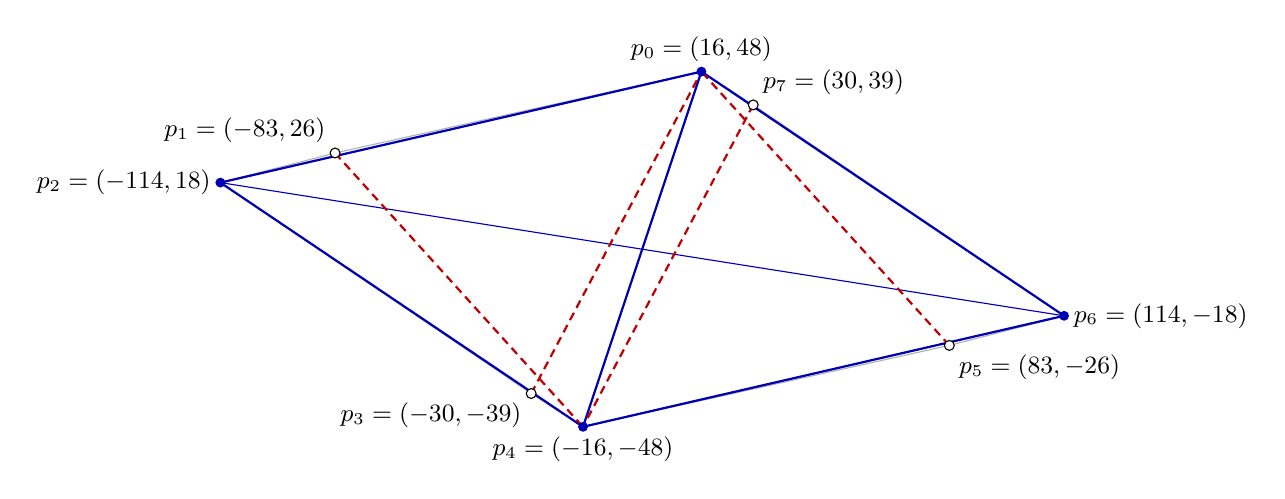
\begin{tikzpicture}[scale=0.047]
  \coordinate (p0) at (16,48);   \coordinate (p1) at (-83,26);
  \coordinate (p2) at (-114,18); \coordinate (p3) at (-30,-39);
  \coordinate (p4) at (-16,-48); \coordinate (p5) at (83,-26);
  \coordinate (p6) at (114,-18); \coordinate (p7) at (30,39);
  \draw[gray!60] (p0)--(p1)--(p2)--(p3)--(p4)--(p5)--(p6)--(p7)--cycle;
  \draw[blue!70!black,thick] (p0)--(p2)--(p4)--(p6)--cycle;
  \draw[blue!70!black,thick] (p0)--(p4);
  \draw[blue!70!black] (p2)--(p6);
  \draw[red!75!black,densely dashed,thick] (p1)--(p4) (p5)--(p0) (p3)--(p0) (p7)--(p4);
  \foreach \p/\pos/\lab in {p0/above/{$p_0=(16,48)$}, p2/left/{$p_2=(-114,18)$}, p4/below/{$p_4=(-16,-48)$}, p6/right/{$p_6=(114,-18)$}}
    {\fill[blue!70!black] (\p) circle (38pt); \node[\pos] at (\p) {\small \lab};}
  \foreach \p/\pos/\lab in {p1/above left/{$p_1=(-83,26)$}, p3/below left/{$p_3=(-30,-39)$}, p5/below right/{$p_5=(83,-26)$}, p7/above right/{$p_7=(30,39)$}}
    {\draw[fill=white] (\p) circle (38pt); \node[\pos] at (\p) {\small \lab};}
\end{tikzpicture}
\caption{The point set $P_\star$ of \cref{thm:tightpair} (to scale),
$r^2=10240$. Solid blue: the only $r$-far $4$-set $\{p_0,p_2,p_4,p_6\}$ and
its six distances; $|p_0p_4|=r$. Each white point is the first far point
$a(\cdot)$ of the blue point before it and is closer than $r$ to another blue
point (dashed red), so it cannot replace anything.}
\label{fig:pstar}
\end{figure}

\begin{theorem}\label{thm:tightpair}
$(\mathrm{TP}_4)$ is false, even at the optimal radius. Let $P_\star$ be the
eight points
\begin{align*}
&p_0=(16,48), &&p_1=(-83,26), &&p_2=(-114,18), &&p_3=(-30,-39),\\
&p_4=(-16,-48), &&p_5=(83,-26), &&p_6=(114,-18), &&p_7=(30,39),
\end{align*}
which are in strictly convex position in this ccw order, and let
$r^2=10240$. Then $\rstar_4(P_\star)=r$, the set $\{p_0,p_2,p_4,p_6\}$ is the
only $r$-far $4$-set, and it contains no tight pair. Consequently
$(\mathrm{TT}_4)$, $(\mathrm{ST}_4)$ and $(\mathrm{AG}_4)$ are false as well.
Moreover, $(\mathrm{TP}_k)$ is false for $k=5$, $6$ and $7$; point sets with
$2k$ points are listed in \cref{app:instances}.
\end{theorem}
\begin{proof}
$P_\star$ is symmetric under $p\mapsto-p$, which maps $p_i$ to $p_{i+4}$. The
squared distances from $p_0,\dots,p_3$ are
\begin{center}\small
\begin{tabular}{@{}c|cccccccc@{}}
 & $p_0$ & $p_1$ & $p_2$ & $p_3$ & $p_4$ & $p_5$ & $p_6$ & $p_7$\\\midrule
$p_0$ & -- & \textbf{10285} & \textbf{17800} & 9685 & \textbf{10240} & 9965 & \textbf{13960} & 277\\
$p_1$ &  & -- & 1025 & 7034 & 9965 & \textbf{30260} & \textbf{40745} & \textbf{12938}\\
$p_2$ &  &  & -- & \textbf{10305} & \textbf{13960} & \textbf{40745} & \textbf{53280} & \textbf{21177}\\
$p_3$ &  &  &  & -- & 277 & \textbf{12938} & \textbf{21177} & 9684\\
\end{tabular}
\end{center}
and the remaining ones follow by symmetry; entries of at least $r^2$ are in
bold. The points at distance at least $r$ from $p_1$ are $p_0,p_5,p_6,p_7$,
and the only pairs among these at distance at least $r$ are $\{p_0,p_6\}$ and
$\{p_6,p_7\}$, so $p_1$ lies in no $r$-far $4$-set; by symmetry neither does
$p_5$. The points at distance at least $r$ from $p_3$ are $p_2,p_5,p_6$, and
$|p_5p_6|<r$, so $p_3$ and, by symmetry, $p_7$ lie in no $r$-far $4$-set
either. Hence the only candidate is $\{p_0,p_2,p_4,p_6\}$, which is $r$-far
with minimum distance $|p_0p_4|=r$; in particular $\rstar_4(P_\star)=r$. From
the table, $a(p_0)=p_1$, $a(p_2)=p_3$, $a(p_4)=p_5$ and $a(p_6)=p_7$. None of
these belongs to the set, so it contains no tight pair.

For $k=5,6,7$ the instances of \cref{app:instances} were verified by
exhaustive enumeration of all $k$-subsets in exact integer arithmetic.
\end{proof}

\paragraph{Anatomy of the counterexample.}
The mechanism is easy to describe (\cref{fig:pstar}). The quadrilateral
$p_0p_2p_4p_6$ is a parallelogram whose short diagonal $p_0p_4$ has length
exactly $r$ and makes an angle of less than $\pi/3$ with the sides $p_0p_2$
and $p_4p_6$. The first far point $a(p_0)=p_1$ sits just outside the side
$p_0p_2$ at distance slightly more than $r$ from $p_0$; the triangle
$p_0p_1p_4$ has two sides of length about $r$ enclosing an angle below
$\pi/3$, so $|p_1p_4|<r$ and $p_1$ is blocked by $p_4$. The point
$a(p_2)=p_3$ sits just before $p_4$ and is slightly closer to $p_0$ than
$p_4$ is, so it is blocked by $p_0$.

More generally, suppose $(\mathrm{TP}_k)$ fails for $(P,r)$ and let
$S=\{s_1,\dots,s_k\}$ be an $r$-far $k$-set in ccw order. By
\cref{lem:arcbasic}, $a_i=a(s_i)$ lies strictly between $s_i$ and $s_{i+1}$,
and since $(S\setminus\{s_{i+1}\})\cup\{a_i\}$ would contain the tight pair
$\{s_i,a_i\}$, each $a_i$ must be closer than $r$ to some $s_j$ with
$j\notin\{i,i+1\}$. So every counterexample contains a convex $2k$-gon
$s_1a_1s_2a_2\cdots s_ka_k$ with $\{s_1,\dots,s_k\}$ $r$-far, $|s_ia_i|\ge r$,
and every $a_i$ blocked in this way; in particular it has at least $2k$
points, and our instances are smallest possible. For $k=3$ no such hexagon
exists by \cref{thm:k3}(ii).


